\documentclass[10pt,twocolumn,letterpaper]{article}



\usepackage{fontspec}
\usepackage[margin=0.75in]{geometry}
\usepackage{amsmath,amssymb,amsfonts,amsthm}
\usepackage{graphicx}
\usepackage{booktabs}
\usepackage{hyperref}
\usepackage{xcolor}
\usepackage{algorithm}
\usepackage{algorithmic}
\usepackage{microtype}
\usepackage{cite}
\usepackage{subcaption}
%\usepackage{multirow}

\hypersetup{
    colorlinks=true,
    linkcolor=blue,
    citecolor=teal,
    urlcolor=magenta
}

\newtheorem{theorem}{Theorem}
\newtheorem{lemma}{Lemma}
\newtheorem{definition}{Definition}

\title{\textbf{Dequantizing Shallow Equivariant Quantum Graph Networks: Periodic Inductive Biases in Molecular Message Passing}}

\author{
    \textbf{Nguyen Trong Luu}, \textbf{Hieu Minh Pham}, \textbf{Anh Quoc Phan}, \textbf{Cho Xuan Do}\thanks{Corresponding author: \texttt{chodx@ptit.edu.vn}} \\
    \textit{Posts and Telecommunications Institute of Technology (PTIT), Hanoi, Vietnam}
}
\date{}

\begin{document}

\maketitle

\begin{abstract}
Parameterized quantum circuits (PQCs) have shown promising results on molecular electronic property prediction, but the source of their advantage over classical baselines remains unclear. We show that this advantage traces not to multi-qubit entanglement but to a classical mechanism: single-qubit rotations natively compute truncated Fourier series, providing a compact periodic basis that monotonic activations cannot efficiently express at low parameter budgets. To exploit this insight, we introduce \textbf{PRISM}, an $\mathrm{E}(3)$-equivariant message-passing GNN that replaces standard activations with periodic sinusoidal (SIREN) internal activations. At identical parameter count ($2{,}527$), PRISM matches or exceeds a 4-qubit PQC across all QM9 electronic targets and outperforms PaiNN on four of six properties. Scaling circuit depth to $L = 16$ layers and qubit counts to $n_q = 8$ confirms that quantum circuits asymptotically match but never exceed PRISM's classical representation, while incurring up to a $540\times$ training slowdown. Across full-scale QM9 ($N = 110{,}000$, 5 seeds, $q_{\mathrm{FDR}} \le 0.055$), the periodic advantage persists and \textit{widens} monotonically from $35.7\%$ to $51.3\%$ as model capacity scales past $100{,}000$ parameters. Our results establish periodic internal activations as a hardware-free inductive bias for molecular geometric deep learning.
\end{abstract}

\section{Introduction}
\label{sec:intro}


Parameterized quantum circuits (PQCs) are leading near-term candidates for practical quantum advantage in machine learning~\cite{Kandala:2017vok, Cerezo:2020mtn}. Molecular property prediction is a natural application domain: molecules live in 3D Euclidean space with continuous $\mathrm{E}(3)$ symmetries that PQCs can naturally respect, and the underlying physics is quantum mechanical~\cite{satorras2022enequivariantgraphneural, thomasTensorFieldNetworks2018}. When integrated into equivariant graph neural networks, shallow PQCs consistently outperform parameter-matched classical baselines on electronic orbital targets such as HOMO, LUMO, and the HOMO-LUMO gap in low-data regimes (Figure~\ref{fig:scaling_law}).

However, the physical mechanism driving this performance remains debated: while prevailing literature attributes gains to multi-qubit entanglement or Hilbert-space expressivity, our systematic ablations across 20 random seeds show that multi-qubit entanglement contributes negligibly. Instead, the mechanism is entirely classical: single-qubit rotations $R_Y(x)$, $R_Z(x)$ natively compute truncated Fourier series~\cite{Schuld:2020enb, Perez-Salinas:2019pjx}, supplying a compact periodic basis that standard monotonic activations ($\tanh$, SiLU) cannot efficiently express at matching parameter budgets. This reflects a representational capacity gap rather than quantum advantage.

This diagnosis is constructive: if the PQC advantage stems from periodicity, we can replicate it classically by placing periodic activations \textit{inside} equivariant message-passing layers. While SIREN~\cite{sitzmann2020siren} introduced sinusoidal activations for implicit neural representations in vision, and existing molecular architectures use trigonometric functions for \textit{input} encodings (spherical harmonics in TFN~\cite{thomasTensorFieldNetworks2018}, NequIP~\cite{batznerE3equivariantGraphNeural2021}, MACE~\cite{batatiaMACEHigherOrder2022}), no prior work has placed periodic activations inside the \textit{hidden layers} of equivariant graph networks. We introduce \textbf{PRISM}, an $\mathrm{E}(3)$-equivariant message-passing GNN that replaces monotonic activations with $\sin(\omega_0 \mathbf{W} \mathbf{x} + \mathbf{b})$ in its edge-processing MLPs. At identical parameter count, PRISM matches or exceeds the PQC on all electronic targets, without quantum hardware.

\paragraph{Contributions.}
\begin{itemize}
    \item We isolate the mechanism of PQC advantage on molecular electronic targets: it traces to single-qubit trigonometric expressivity, not multi-qubit entanglement (Section~\ref{sec:mechanism}).
    \item We introduce \textbf{PRISM}, the first equivariant message-passing GNN with periodic sinusoidal \textit{internal} activations, which matches or exceeds the PQC at iso-parameter parity and outperforms PaiNN on four of six QM9 targets (Section~\ref{sec:periodic_egnn}).
    \item We prove classical sufficiency across circuit scaling regimes: scaling PQC depth to $L = 16$ layers and qubit width to $n_q = 8$ confirms that deep quantum entanglement yields zero marginal advantage over PRISM's two-layer periodic edge representation, while classical execution delivers a $540\times$ training speedup (Section~\ref{sec:depth_qubit_scaling}).
    \item We demonstrate that the periodic advantage persists at full scale ($N = 110{,}000$, 5 seeds, $q_{\mathrm{FDR}} \le 0.055$; $p = 0.0035$ on HOMO, $p = 0.0424$ on LUMO, $p = 0.0547$ on Gap) and \textit{widens monotonically} from $35.7\%$ to $51.3\%$ as model capacity scales to the standard medium-capacity regime of $100{,}127$ parameters (Section~\ref{sec:param_scaling}).
    \item We provide a rigorous statistical methodology (factorial ablation, Fourier spectral validation, and Benjamini-Hochberg FDR correction across 48 hypotheses) applicable to future QML benchmarking (Section~\ref{sec:init_ablation}, Supplementary Table~S3 in SM~B, SM~D).
\end{itemize}

\begin{figure*}[t]
    \centering
    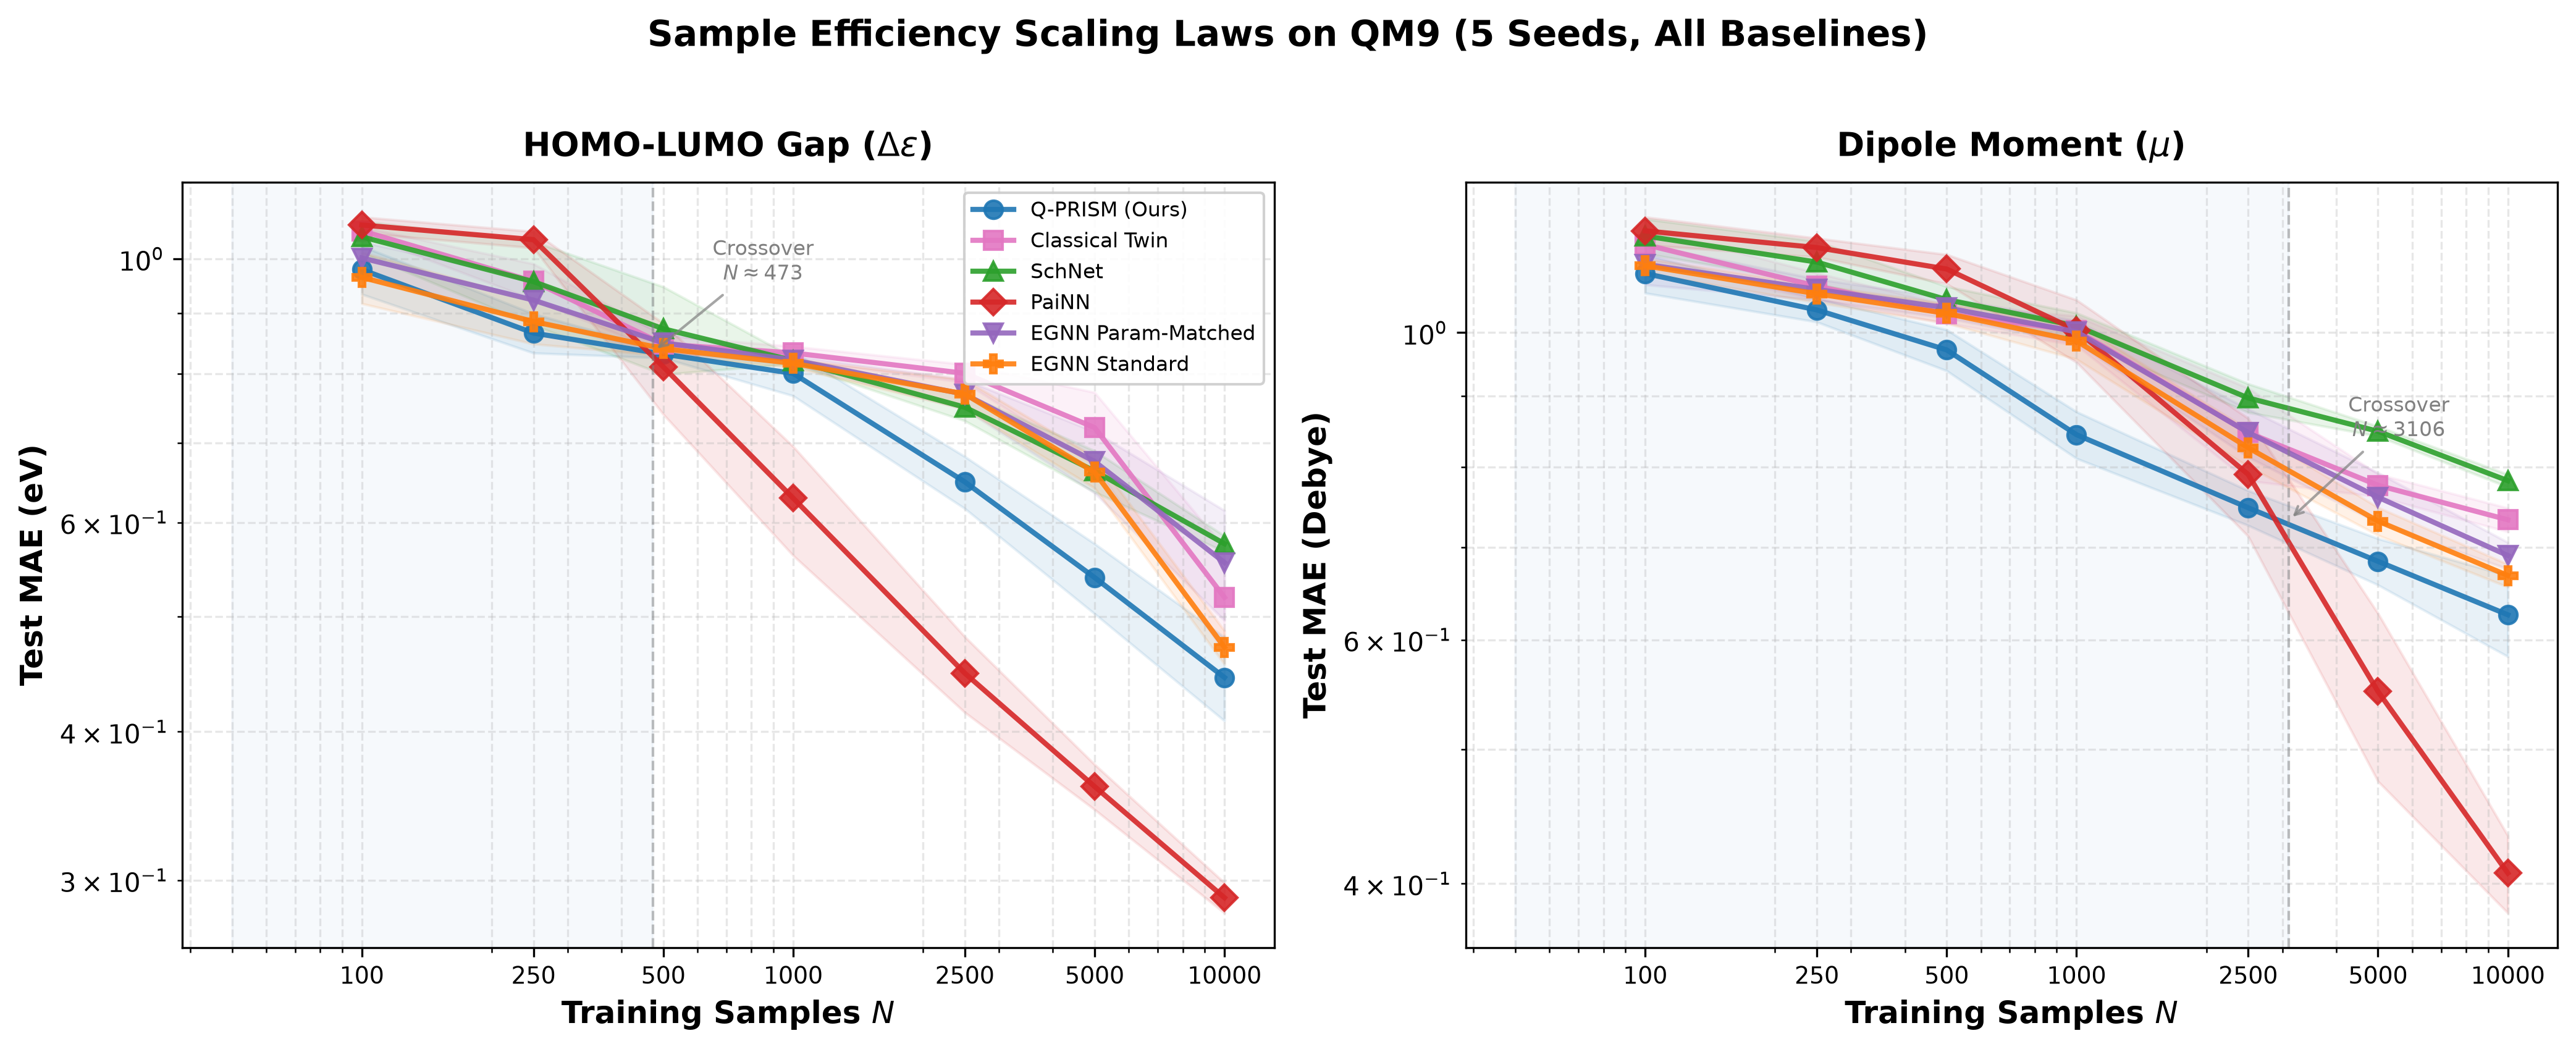
\includegraphics[width=0.88\textwidth]{figures/figure1_scaling_law.png}
    \caption{\textbf{Sample Efficiency Scaling Laws on QM9 across Sample Sizes $N \in [100, 10{,}000]$:} Log-log scaling curves for HOMO-LUMO gap $\Delta\epsilon$ (left, eV) and Dipole Moment $\mu$ (right, Debye) across 5 independent random seeds (mean $\pm$ std). Q-PRISM ($2{,}527$\,p) is benchmarked against Classical Twin ($\tanh$, $2{,}527$\,p), SchNet ($2{,}473$\,p), PaiNN ($2{,}721$\,p), EGNN Param-Matched ($2{,}497$\,p), and EGNN Standard ($4{,}289$\,p). In data-scarce regimes ($N \le 500$), Q-PRISM outperforms all baselines. As sample size grows, PaiNN's coupled scalar-vector representation crosses over Q-PRISM at $N \approx 473$ for Gap and $N \approx 3{,}106$ for Dipole Moment, while Q-PRISM consistently maintains an advantage over scalar equivariant baselines (EGNN, SchNet).}
    \label{fig:scaling_law}
\end{figure*}

\section{Related Work}
\label{sec:related}

\paragraph{Classical Geometric Deep Learning.}
Equivariant GNNs for molecular property prediction have achieved strong accuracy on quantum chemistry benchmarks (see No{\'e} et al.~\cite{Noe:2019yup} for a review). Representative architectures include invariant message-passing models (EGNN~\cite{satorras2022enequivariantgraphneural}, SchNet~\cite{schütt2017schnetcontinuousfilterconvolutionalneural}, PhysNet~\cite{unkePhysNetNeuralNetwork2019}), directional and angular architectures (DimeNet++~\cite{klicperaFastUncertaintyAwareDirectional2020}, GemNet~\cite{klicperaGemNetUniversalDirectional2021}, PaiNN~\cite{schuttEquivariantMessagePassing2021}), higher-order tensor methods (TFN~\cite{thomasTensorFieldNetworks2018}, NequIP~\cite{batznerE3equivariantGraphNeural2021}, MACE~\cite{batatiaMACEHigherOrder2022}, Equiformer~\cite{liao2023equiformer}), and scalable equivariant frameworks (TorchMD-Net~\cite{tholke2022torchmdnet}, Allegro~\cite{musaelianLearningLocalEquivariant2022}, LEFTNet~\cite{duNewPerspectiveBuilding2023}). The MPNN framework of Gilmer et al.~\cite{gilmer2017neural} unifies most of these under a common message-passing formalism. Yet all share a common design choice: monotonic, locally-linear activation functions (SiLU, Swish, or shifted softplus) in their internal message-passing and node-update MLPs. We challenge this default.

\paragraph{Spectral Bias and Periodic Activations.}
In deep learning theory, Rahaman et al.~\cite{rahaman2019spectral} proved that standard neural networks exhibit \textit{spectral bias}: gradient descent prioritizes fitting low-frequency Fourier components, with high-frequency Fourier amplitudes decaying rapidly as $\mathcal{O}(\|k\|^{-(d+1)})$.
Tancik et al.~\cite{tancik2020fourier} analyzed this via Neural Tangent Kernel (NTK) theory, demonstrating that coordinate MLPs fail to represent fine spatial structures unless inputs are mapped to Fourier features.
Sitzmann et al.~\cite{sitzmann2020siren} introduced SIREN (Sinusoidal Representation Networks), demonstrating that periodic activation functions ($\sin(\omega_0 W x + b)$) combined with a principled initialization scheme ($\omega_0$-scaled uniform distribution) completely bypass spectral bias and allow stable training of arbitrary derivative orders.
While SIREN is standard for implicit neural representations in vision~\cite{sitzmann2020siren}, periodic \textit{internal} activations have not previously appeared inside the message-passing MLPs of equivariant graph neural networks. Existing geometric models employ trigonometric functions only for \textit{input spatial encodings}, such as spherical Bessel radial bases in DimeNet++~\cite{klicperaFastUncertaintyAwareDirectional2020} or spherical harmonics in NequIP~\cite{batznerE3equivariantGraphNeural2021} and MACE~\cite{batatiaMACEHigherOrder2022}, leaving all downstream layer activations monotonic.

\paragraph{Dequantization and Fundamental Limits of QML.}
Recent studies question whether PQC advantages reflect quantum resources. Huang et al.~\cite{Huang:2021qml} showed that QML model power depends on inductive bias alignment with the data, not quantum hardware per se; Schuld~\cite{Schuld:2021kernel} proved that supervised variational models are formally kernel methods. Empirically, Schreiber et al.~\cite{Schreiber:2022roq} showed that PQCs compute truncated Fourier series matchable by classical surrogates, K\"ubler et al.~\cite{kubler2021inductive} traced quantum kernel performance to inductive bias rather than hardware, and Pegg et al.~\cite{pegg2026isoqgnn} showed that iso-parameter classical twins match quantum models on HOMO-LUMO gap prediction. Landman et al.~\cite{landman2023approximating} established that data re-uploading PQCs are multi-dimensional truncated Fourier series approximable via Random Fourier Features in polynomial sample complexity. This is theoretically grounded: Cerezo, Holmes et al.~\cite{Cerezo:2023nqf} established the \textit{trainability-simulability dilemma}, showing that PQCs that avoid barren plateaus~\cite{Cerezo:2020mtn, McClean:2018jps} frequently reside within classically simulable complexity classes, while scaling to deeper, highly entangled circuits risks exponential concentration~\cite{Thanasilp:2022agd}, forcing quantum kernels to trivial constants. Jerbi et al.~\cite{Jerbi:2021qnz} characterized the demanding structural conditions needed to maintain advantage over classical learners. Following Tang's dequantization framework~\cite{Tang:2018lmw}, our approach isolates the precise mechanism of apparent PQC performance and replicates it classically.

\paragraph{Equivariant Quantum Machine Learning.}
Formal frameworks incorporate symmetry constraints into parameterized quantum circuits.
Meyer et al.~\cite{meyer2023exploiting} developed a symmetry group framework for constructing equivariant PQCs, showing that enforcing group symmetries reduces the circuit's effective hypothesis space to physically relevant subspaces, improving sample efficiency and generalization.
Skolik et al.~\cite{skolik2023equivariant} showed that equivariant quantum circuits achieve better generalization on symmetric learning tasks with fewer trainable parameters.
Q-PRISM's $\mathrm{E}(3)$ equivariance is achieved at the \textit{graph architecture level} (through invariant edge inputs and equivariant coordinate updates) rather than through symmetric circuit design, complementing these circuit-level approaches. PRISM inherits the same graph-level equivariance guarantees (Theorem~\ref{thm:equivariance}) without quantum hardware.

\section{Q-PRISM: Equivariant Quantum Graph Architecture}
\label{sec:method}

\begin{figure*}[t]
    \centering
    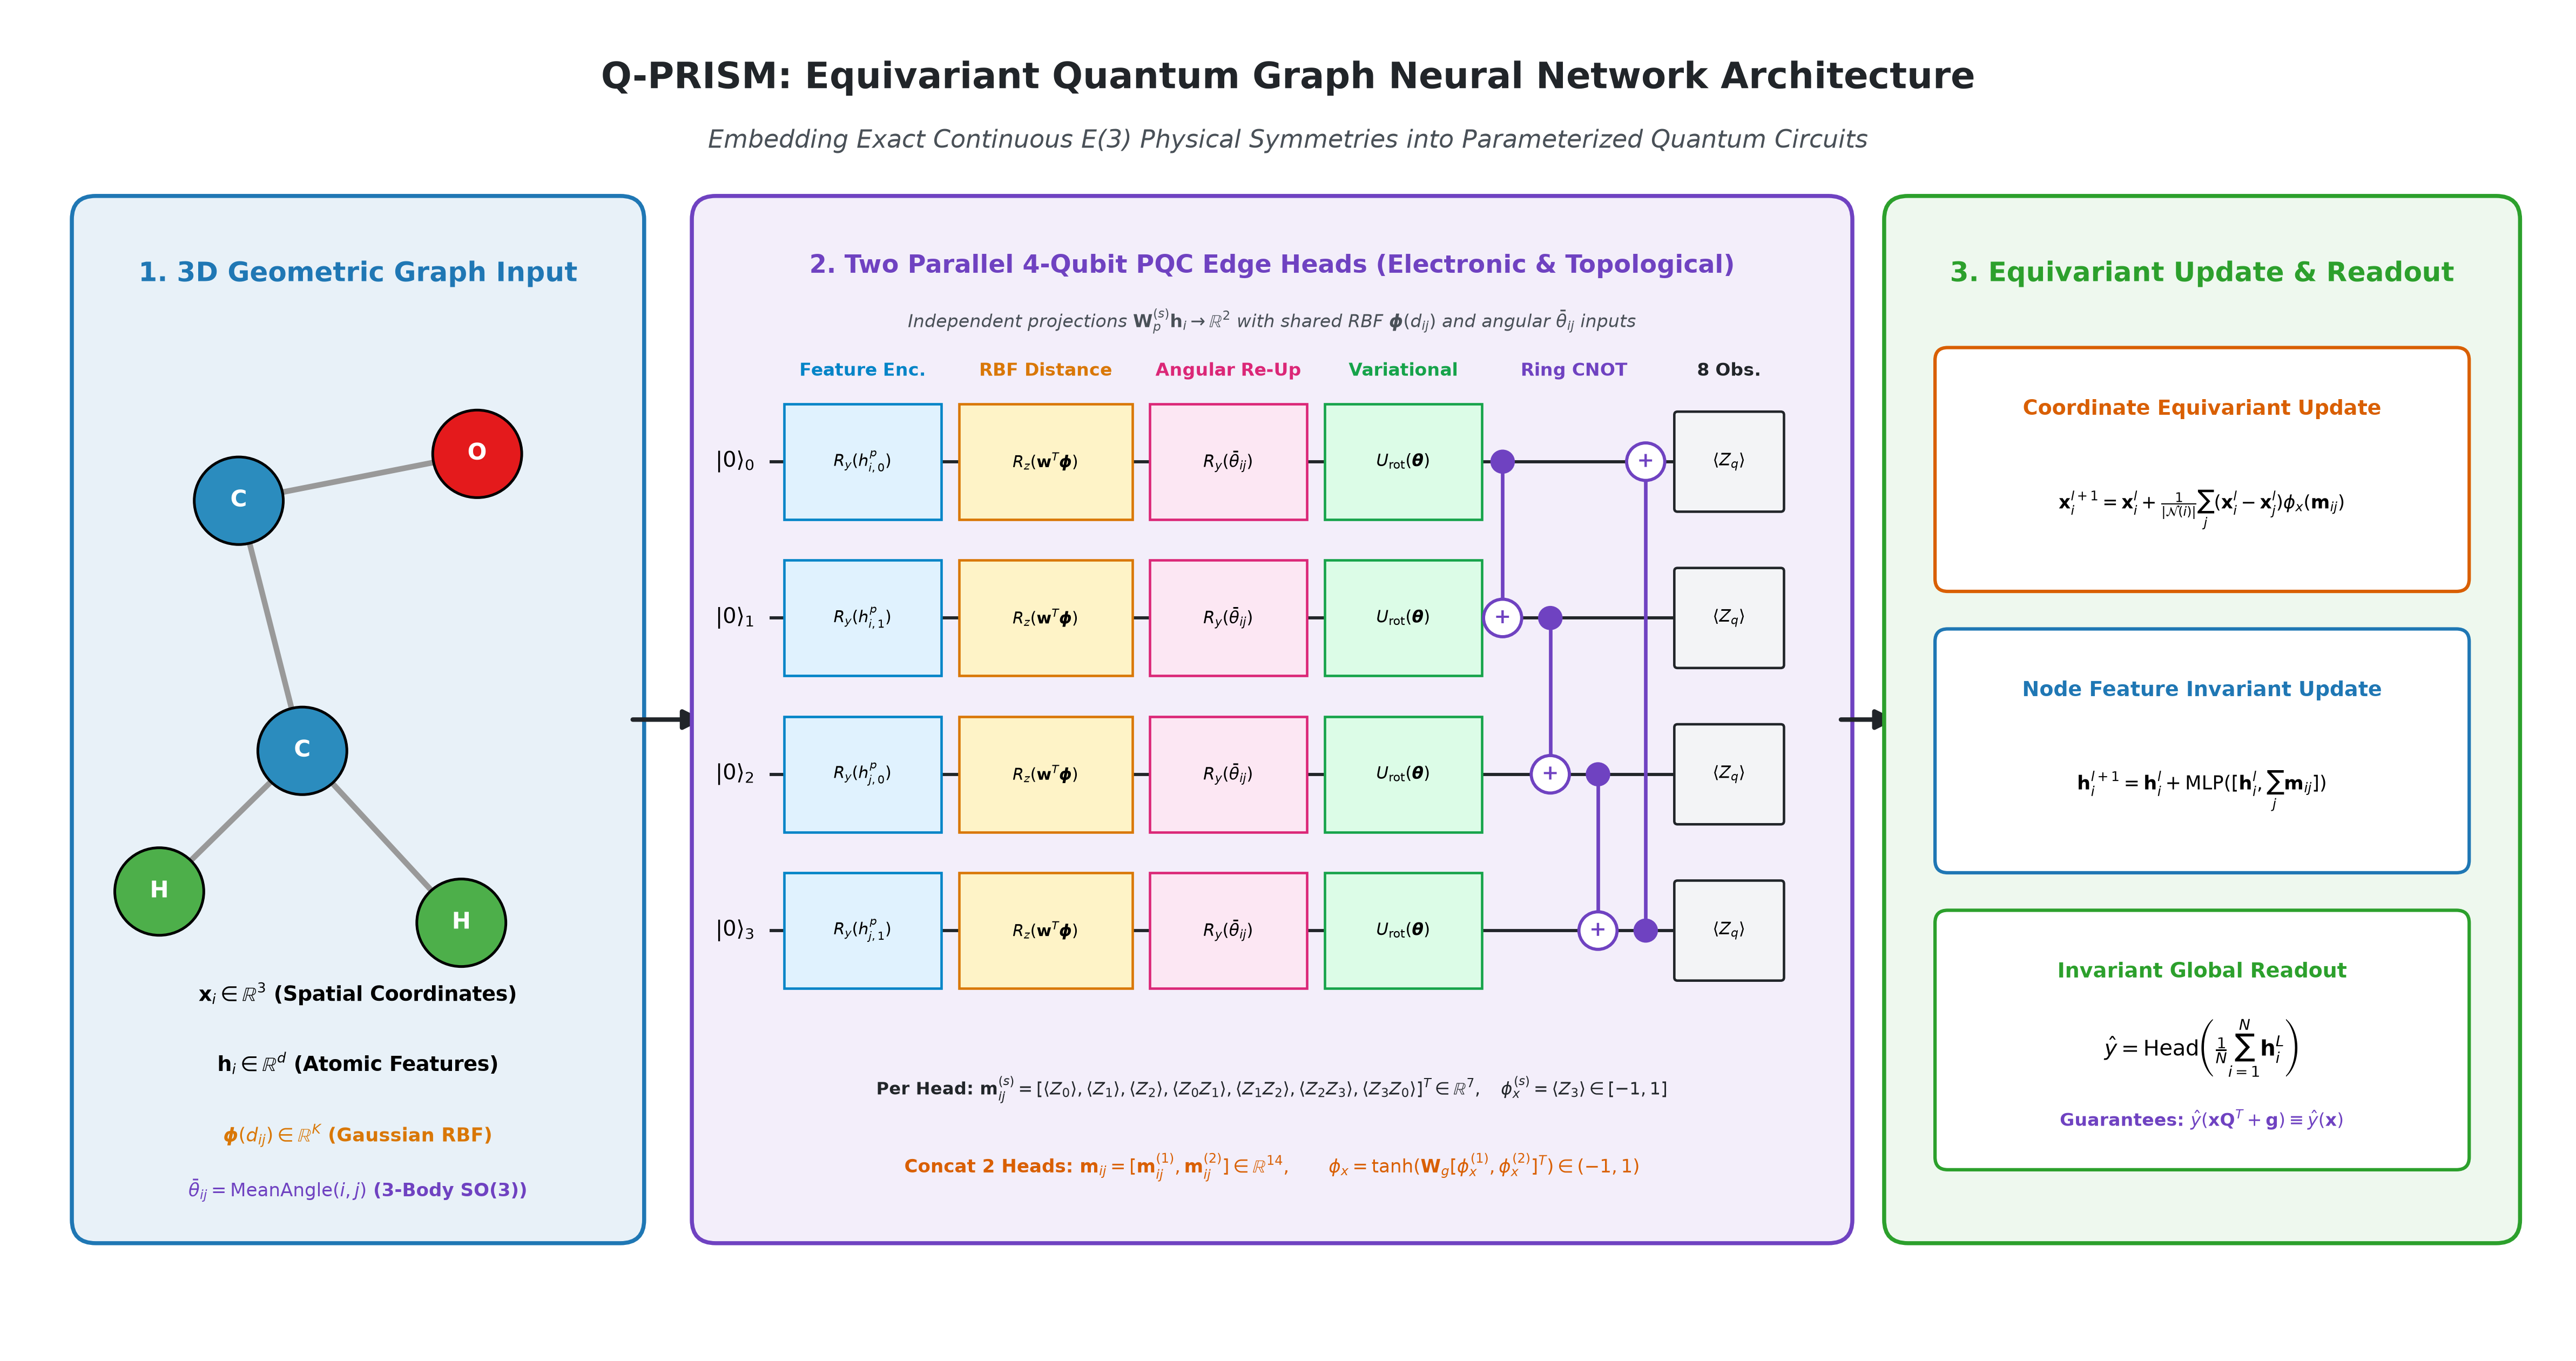
\includegraphics[width=\textwidth]{figures/figure_architecture.png}
    \caption{\textbf{Q-PRISM Architecture:} (1) Input 3D molecular graph with invariant RBF distance features $\boldsymbol{\phi}(d_{ij})$ and SO(3)-invariant bond angles $\bar{\theta}_{ij}$. (2) Two parallel 4-qubit PQC heads (Electronic \& Topological) with multi-frequency RBF distance re-uploading, angular encoding, variational rotations, and ring CNOT entanglement. (3) 8-observable readout per head: 4 single-qubit $\langle Z_q \rangle$ + 4 correlators $\langle Z_i Z_j \rangle$. (4) $\tanh$-gated equivariant coordinate updates and invariant feature message passing yielding global molecular property predictions.}
    \label{fig:architecture}
\end{figure*}

\subsection{Quantum Edge Convolution}
\label{sec:quantum_edge}

As illustrated in Figure~\ref{fig:architecture}, let a 3D molecule be represented as a graph $\mathcal{G} = (\mathcal{V}, \mathcal{E}, \mathbf{x}, \mathbf{h})$, where each atom $i \in \mathcal{V}$ has spatial coordinates $\mathbf{x}_i \in \mathbb{R}^3$ and invariant atomic feature vector $\mathbf{h}_i \in \mathbb{R}^{d_{\mathrm{in}}}$. Edges $(i, j) \in \mathcal{E}$ connect interacting atomic pairs within a radius cutoff, defining the neighborhood $\mathcal{N}(i) = \{j : (i, j) \in \mathcal{E}\}$. The squared Euclidean distance is:
\begin{equation}
    d_{ij} = \|\mathbf{x}_i - \mathbf{x}_j\|^2 \in \mathbb{R}_{\ge 0}
\end{equation}

\paragraph{Gaussian RBF Distance Expansion.}
Rather than encoding raw distances via a single scalar weight $w_d^{(l)} \cdot d_{ij}$, we expand distances into a multi-frequency Gaussian radial basis \cite{schütt2017schnetcontinuousfilterconvolutionalneural}:
\begin{equation}
    \phi_k(d_{ij}) = \exp\left(-\gamma_k (d_{ij} - \mu_k)^2\right), \quad k = 1, \ldots, K
    \label{eq:rbf}
\end{equation}
where $\mu_k$ are evenly spaced centers in $[0, 10]$~\AA$^2$ and $\gamma_k$ are learnable inverse widths. Under the Fourier analysis of data re-uploading \cite{Perez-Salinas:2019pjx, Schuld:2020enb}, this transforms the PQC into a truncated $K$-term Fourier approximator for molecular potential surfaces.

\paragraph{Multi-Head Design.}
Following multi-head attention designs, we use two parallel PQC heads (\textit{Electronic} and \textit{Topological}). Each head uses an independent feature projection $\mathbf{W}_p^{(s)}: \mathbb{R}^{d_{\mathrm{hidden}}} \to \mathbb{R}^2$ to direct distinct feature subspaces into its respective quantum circuit:
\begin{equation}
    \mathbf{h}_i^{p,(s)} = \mathbf{W}_p^{(s)} \mathbf{h}_i, \quad s \in \{1, 2\}
\end{equation}
Both heads share the same RBF distance features and angular inputs but process them through independent PQC parameter sets.

\paragraph{4-Qubit Parameterized Quantum Circuit.}
For each head $s \in \{1, 2\}$ and directed edge $(i, j)$, the edge input vector $\mathbf{u}_{ij}^{(s)} = [\mathbf{h}_i^{p,(s)\top}, \mathbf{h}_j^{p,(s)\top}, \boldsymbol{\phi}(d_{ij})^\top, \bar{\theta}_{ij}]^\top \in \mathbb{R}^{4+K+1}$ is processed by a 4-qubit circuit initialized in $|0\rangle^{\otimes 4}$. As diagrammed in Figure~\ref{fig:architecture}(2), the state evolves through $L$ variational layers via chronological operator composition, $|\psi_{ij}^{(s)}\rangle = \left(\prod_{l=L}^1 U^{(l)}(\mathbf{u}_{ij}^{(s)}, \boldsymbol{\theta}_l)\right) |0\rangle^{\otimes 4}$. Each variational layer $U^{(l)}$ composes multi-axis single-qubit phase injections with a cyclic entangling ring:
\begin{align}
    U^{(l)}(\mathbf{u}_{ij}^{(s)}, \boldsymbol{\theta}_l) &= \mathcal{W}_{\mathrm{ring}} \bigotimes_{q=0}^3 \Big[ R_{ZYX}(\boldsymbol{\theta}_{l,q}) \, R_y(\bar{\theta}_{ij}) \nonumber \\
    &\quad \cdot R_z\!\left(\sum_{k=1}^K w_{d,q,k}^{(l)} \phi_k(d_{ij})\right) R_y(\tilde{h}_{ij,q}^{(s)}) \Big]
    \label{eq:layer_unitary}
\end{align}
where operations evaluate chronologically from right to left. Here, $\tilde{\mathbf{h}}_{ij}^{(s)} = [\mathbf{h}_i^{p,(s)\top}, \mathbf{h}_j^{p,(s)\top}]^\top \in \mathbb{R}^4$ injects projected atom features into the initial Pauli-$Y$ phase on qubit $q \in \{0, \dots, 3\}$; the $K$-channel Gaussian RBF vector $\boldsymbol{\phi}(d_{ij})$ is linearly projected via trainable weights $\mathbf{w}_{d,q}^{(l)} \in \mathbb{R}^K$ into the Pauli-$Z$ phase, injecting a truncated Fourier distance basis; $\bar{\theta}_{ij}$ injects the $\mathrm{O}(3)$-invariant mean bond angle into the second Pauli-$Y$ rotation; $R_{ZYX}(\boldsymbol{\theta}_{l,q}) = R_z(\theta_{l,q,2}) R_y(\theta_{l,q,1}) R_x(\theta_{l,q,0})$ provides a universal single-qubit Euler rotation with 3 trainable parameters per qubit ($12$ per layer); and $\mathcal{W}_{\mathrm{ring}} = \prod_{q=0}^3 \mathrm{CX}_{q \to (q+1)\bmod 4}$ circulates quantum phase information across the 4-qubit register ($\mathrm{CX}_{c \to t}$ denotes a controlled-NOT gate with control qubit $c$ and target qubit $t$).

Equation~(\ref{eq:layer_unitary}) illustrates the dequantization mechanism: all physical data channels (atomic identities, interatomic distances, and 3-body angles) are packed strictly into local single-qubit phase rotations, confirming that data re-uploading natively constructs independent multi-channel Fourier series before $\mathcal{W}_{\mathrm{ring}}$ couples them.

\paragraph{3-Body SO(3)-Invariant Angular Encoding.}
For each edge $(i, j)$, we compute the mean bond angle $\bar{\theta}_{ij}$ across all third atoms $k \in \mathcal{N}(i), k \neq j$ via vectorized $O(E)$ operations:
\begin{align}
    \bar{\cos}_{ij} &= \frac{\hat{\mathbf{r}}_{ij} \cdot \sum_{k \in \mathcal{N}(i)} \hat{\mathbf{r}}_{ik} - 1}{\deg(i) - 1}, \label{eq:angle} \\
    \bar{\theta}_{ij} &= \arccos\!\left(\mathrm{clamp}(\bar{\cos}_{ij}, -1, 1)\right) \nonumber
\end{align}
where $\hat{\mathbf{r}}_{ij} = (\mathbf{x}_j - \mathbf{x}_i) / \|\mathbf{x}_j - \mathbf{x}_i\|$. For monovalent atoms ($\deg(i) = 1$), the denominator in Eq.~(\ref{eq:angle}) is clamped to $1$, yielding $\bar{\theta}_{ij} = \pi/2$ as an uninformative default. This is strictly $\mathrm{O}(3)$-invariant since $\cos \theta_{ijk} = \hat{\mathbf{r}}_{ij} \cdot \hat{\mathbf{r}}_{ik}$ depends only on inner products of relative vectors: $(\mathbf{Q}\hat{\mathbf{r}}_{ij})^\top (\mathbf{Q}\hat{\mathbf{r}}_{ik}) = \hat{\mathbf{r}}_{ij}^\top \mathbf{Q}^\top \mathbf{Q} \hat{\mathbf{r}}_{ik} = \hat{\mathbf{r}}_{ij}^\top \hat{\mathbf{r}}_{ik}$.

\paragraph{Angular Degeneracy of Mean Pooling.}
Mean-angle pooling can map distinct coordination environments to similar scalar values (e.g., sp$^3$ vs.\ sp$^2$ carbons differ by only $\sim 10^\circ$). In practice, the node embedding and RBF distance channels provide sufficient disambiguation for QM9's rigid organic molecules; extending to diverse coordination chemistry (e.g., transition metal complexes) requires per-triplet angular expansion~\cite{klicperaFastUncertaintyAwareDirectional2020, klicperaGemNetUniversalDirectional2021} (see Limitation 2, SM~H).

\paragraph{Entanglement Correlator Readout.}
Each head produces 8 observables from the output state $|\psi_{ij}^{(s)}\rangle$: 4 single-qubit expectations $\langle Z_q \rangle_{ij}^{(s)}$ and 4 ring correlators $\langle Z_q Z_{(q+1)\bmod 4} \rangle_{ij}^{(s)}$ for $q \in \{0, 1, 2, 3\}$. The 8 observables are partitioned into coordinate and feature channels:
\begin{align}
    \mathbf{m}_{ij}^{(s)} &= \big[\langle Z_0 \rangle, \langle Z_1 \rangle, \langle Z_2 \rangle, \nonumber \\
    &\quad \langle Z_0 Z_1 \rangle, \langle Z_1 Z_2 \rangle, \langle Z_2 Z_3 \rangle, \langle Z_3 Z_0 \rangle\big]^\top \in \mathbb{R}^7, \\
    \phi_x^{(s)} &= \langle Z_3 \rangle_{ij}^{(s)} \in [-1, 1].
\end{align}
Qubit 3 is designated as the coordinate-update observable because it is maximally distant from the feature-encoding qubits (0, 1) in the ring CNOT topology, so $\phi_x^{(s)}$ carries an entanglement-processed signal rather than raw input rotations.

The two heads' messages are concatenated: $\mathbf{m}_{ij} = [\mathbf{m}_{ij}^{(1)}, \mathbf{m}_{ij}^{(2)}] \in \mathbb{R}^{14}$.

\subsection{Equivariant Message Passing}
\label{sec:message_passing}

The per-head coordinate observables $\phi_x^{(1)}, \phi_x^{(2)}$ from \S\ref{sec:quantum_edge} are combined into a single gated scalar via $\tanh$ activation, bounding each coordinate update to $(-1, 1)$:
\begin{equation}
    \phi_x(\mathbf{m}_{ij}) = \tanh\!\left(\mathbf{W}_g \left[\phi_x^{(1)}, \phi_x^{(2)}\right]^T\right) \in (-1, 1)
\end{equation}
\begin{equation}
    \mathbf{x}_i^{l+1} = \mathbf{x}_i^l + \frac{1}{|\mathcal{N}(i)|} \sum_{j \in \mathcal{N}(i)} (\mathbf{x}_i^l - \mathbf{x}_j^l) \cdot \phi_x(\mathbf{m}_{ij})
    \label{eq:coord_update}
\end{equation}

\paragraph{Invariant Feature Message Passing.}
Edge messages are aggregated per node and combined with the current features through a residual MLP update:
\begin{align}
    \mathbf{m}_i &= \sum_{j \in \mathcal{N}(i)} \mathbf{m}_{ij} \\
    \mathbf{h}_i^{l+1} &= \mathbf{h}_i^l + \mathrm{MLP}\left([\mathbf{h}_i^l, \mathbf{m}_i]\right)
    \label{eq:feat_update}
\end{align}

\subsection{Classical Dequantization: PRISM}
\label{sec:periodic_egnn}


To test whether the PQC's performance originates from quantum mechanical properties or from classical trigonometric expressivity, we construct structurally matched classical surrogates following the empirical dequantization framework~\cite{Tang:2018lmw, Schreiber:2022roq, pegg2026isoqgnn}.
We use ``dequantization'' in the heuristic, empirical sense of Schreiber et al.~\cite{Schreiber:2022roq}: constructing a classical model with structurally analogous hypothesis class and demonstrating equal or superior performance (see SM~D for detailed discussion of terminology, dimensionality mismatch, and activation choice).

\paragraph{Classical Twin ($\tanh$-MLP).}
The standard classical twin uses a two-layer MLP with sigmoid-family activations:
\begin{equation}
    \mathbf{o}_{ij}^{(s)} = \tanh\left(\mathbf{W}_2 \operatorname{SiLU}(\mathbf{W}_1 \mathbf{u}_{ij}^{(s)} + \mathbf{b}_1)\right)
\end{equation}
where $\mathbf{W}_1 \in \mathbb{R}^{4 \times 13}$ and $\mathbf{W}_2 \in \mathbb{R}^{8 \times 4}$ (without bias). The trainable parameter budget per head is exactly $4 \times (13 + 1) + 4 \times 8 = 88$, matching the 88 parameters of the 4-qubit PQC ($24$ rotation angles $+ 64$ distance re-uploading weights) for an exact model-wide match of $2{,}527$ parameters.
\paragraph{PRISM (SIREN Periodic Twin).}
To overcome the representational limits of monotonic activations at low parameter budgets~\cite{rahaman2019spectral, sitzmann2020siren}, we replace the monotonic activation with a periodic sinusoidal non-linearity with SIREN initialization~\cite{sitzmann2020siren}:
\begin{equation}
    \mathbf{o}_{ij}^{(s)} = \tanh\left(\mathbf{W}_2 \sin\left(\omega_0 (\mathbf{W}_1 \mathbf{u}_{ij}^{(s)} + \mathbf{b}_1)\right)\right)
\end{equation}
with frequency hyperparameter $\omega_0 = 30.0$ fixed \textit{a priori} following Sitzmann et al.~\cite{sitzmann2020siren}. An extended 9-point grid sweep across $\omega_0 \in [1, 100]$ (10 seeds, SM~D, Table~S5, Figure~S5) confirms that the periodic advantage remains stable across frequencies, with an optimal physical resonance band emerging at $\omega_0 \approx 50$ (yielding a $-38.9\%$ error reduction vs.\ the Classical Twin on Gap).
Following Sitzmann et al.~\cite{sitzmann2020siren}, weights are initialized as:
\begin{equation}
    \mathbf{W}_1 \sim \mathcal{U}\left(-\frac{1}{d_{\mathrm{edge}}}, \frac{1}{d_{\mathrm{edge}}}\right), \quad \mathbf{W}_2 \sim \mathcal{U}\left(-\frac{\sqrt{6/d_h}}{\omega_0}, \frac{\sqrt{6/d_h}}{\omega_0}\right)
\end{equation}
where $d_{\mathrm{edge}} = 13$ and $d_h = 4$.
This guarantees uniform variance propagation across periodic activations, preserving oscillatory angular gradients without numerical saturation. The trainable parameter count remains identical at exactly $2{,}527$ parameters.
\paragraph{Fourier Feature Twin (RFF).}
As an alternative baseline, we implement Random Fourier Features (RFF) following Tancik et al.~\cite{tancik2020fourier}:
$\gamma(\mathbf{u}) = [\cos(2\pi \mathbf{B}\mathbf{u}), \sin(2\pi \mathbf{B}\mathbf{u})]^T$, where $\mathbf{B} \in \mathbb{R}^{13 \times 4}$ is a fixed Gaussian random matrix ($\sigma = 10.0$), followed by a linear projection matching $2{,}515$ parameters ($\Delta = -12$).

Because all inputs $\mathbf{u}_{ij}^{(s)}$ are strictly $\mathrm{O}(3)$-invariant, Theorem~\ref{thm:equivariance} applies identically to PRISM, Classical Twin ($\tanh$), and Fourier Feature twins, guaranteeing exact machine-precision $\mathrm{E}(3)$ equivariance for all classical variants.
\subsection{Theoretical Guarantees}
\label{sec:theory}

\begin{theorem}[$\mathrm{E}(3)$ Equivariance of Q-PRISM Layer]
\label{thm:equivariance}
Let $\mathcal{T}_{\mathbf{Q}, \mathbf{g}}(\mathbf{x}) = \mathbf{x} \mathbf{Q}^T + \mathbf{g}$ denote an arbitrary continuous Euclidean transformation with rotation/reflection $\mathbf{Q} \in \mathrm{O}(3)$ and translation $\mathbf{g} \in \mathbb{R}^3$.\footnote{We adopt a row-vector convention throughout: coordinates are stored as $\mathbf{x}_i \in \mathbb{R}^{1 \times 3}$ (row vectors), so the transformation is $\mathbf{x} \mathbf{Q}^T + \mathbf{g}$ rather than $\mathbf{Q}\mathbf{x} + \mathbf{g}$. This matches PyTorch's default batch-of-row-vectors layout.} Then for the Q-PRISM layer defined in Eqs.~(\ref{eq:coord_update}--\ref{eq:feat_update}):
\begin{align}
    \mathbf{h}_i^{l+1}(\mathcal{T}_{\mathbf{Q}, \mathbf{g}}(\mathbf{x}), \mathbf{h}) &= \mathbf{h}_i^{l+1}(\mathbf{x}, \mathbf{h}) \quad (\text{Invariance}) \\
    \mathbf{x}_i^{l+1}(\mathcal{T}_{\mathbf{Q}, \mathbf{g}}(\mathbf{x}), \mathbf{h}) &= \mathcal{T}_{\mathbf{Q}, \mathbf{g}}(\mathbf{x}_i^{l+1}(\mathbf{x}, \mathbf{h})) \quad (\text{Equivariance})
\end{align}
\end{theorem}

The proof follows from the $\mathrm{O}(3)$-invariance of all PQC inputs ($d_{ij}$, $\bar{\theta}_{ij}$, $\mathbf{h}_i$) and the equivariant structure of the coordinate update (Eq.~\ref{eq:coord_update}); see SM~C for the full derivation. Numerical testing with random $\mathrm{O}(3)$ rotations confirms equivariance errors $\le 2.38 \times 10^{-7}$. Algorithm pseudocode is provided in SM~C.

\section{Experimental Evaluation}
\label{sec:experiments}

\subsection{Benchmark Setup}

We benchmark Q-PRISM on the standard QM9 dataset \cite{ramakrishnan2014quantum}, containing $130{,}831$ small organic molecules with quantum electronic properties computed at the B3LYP/6-31G(2df,p) level of DFT.
We evaluate across 6 physical targets using 5 independent random seeds ($42$--$46$) on $N = 1{,}000$ training molecules and $500$ test molecules.
We select targets that span three distinct physical mechanisms: intensive electronic properties (HOMO, LUMO, Gap), which probe angular orbital overlaps central to our spectral bias hypothesis; extensive electrostatic properties (dipole moment $\mu$, polarizability $\alpha$), which test coordinate-dependent charge distribution; and extensive thermodynamic energy ($U_0$). We note that KS-DFT LUMO energies, unlike HOMO energies (which approximate ionization potentials via the Kohn-Sham analog of Koopmans' theorem), lack strict physical interpretation and are highly basis-set dependent; LUMO results should be interpreted with this caveat. The remaining QM9 properties ($U$, $H$, and $G$) derive linearly from $U_0$ through thermal and entropic corrections, making separate comparisons redundant. Vibrational properties ($\text{ZPVE}$ and $C_v$) fall outside the capacity of compact $\sim 2{,}500$-parameter models.
The $1{,}000 / 500$ split (a 2:1 ratio) represents a standard protocol for low-data chemical benchmarking, providing sufficient statistical power for paired comparisons while maintaining simulation tractability across 8 models and multi-seed sweeps.
Complete training hyperparameters (optimizer, learning rate, scheduler, batch size, early stopping, and computational resources) are provided in SM~A, Table~S1.
All experiments use 5 independent random seeds controlling both initialization and data splits; the 20-seed ablation (Section~\ref{sec:mechanism}) confirms robustness. Statistical details (seed protocol, power analysis, Wilcoxon tests) are in SM~B.

We evaluate an 8-model hierarchy: (i) \textit{Classical Twin} ($\tanh$-MLP, $2{,}527$\,p), (ii) \textit{PRISM} (SIREN, $2{,}527$\,p), (iii) \textit{RFF Twin} ($2{,}515$\,p), (iv--v) SchNet ($2{,}473$\,p) and PaiNN ($2{,}721$\,p), (vi--vii) iso-parameter and standard EGNN, and (viii) a non-equivariant GNN control.

\begin{table*}[t]
\centering
\footnotesize
\setlength{\tabcolsep}{2.5pt}
\caption{\textbf{Multi-Target QM9 Benchmark Across 8 Models with Dequantized Trigonometric Twins and SOTA Baselines} ($N = 1{,}000$, Mean $\pm$ Std across 5 Seeds). Best result per row in \textbf{bold}. For reference, chemical accuracy is $0.043$\,eV ($1$\,kcal/mol); all models operate well above this threshold in the parameter-constrained regime. Statistical significance of PRISM (SIREN) vs.\ Classical Twin ($\tanh$) under Benjamini-Hochberg FDR multiplicity correction ($m = 48$ hypotheses): $^{\dagger}q < 0.05$, $^{\dagger\dagger}q < 0.01$. Significance of Q-PRISM vs.\ Classical Twin ($\tanh$): $^*p < 0.05$, $^{**}p < 0.01$ (unadjusted paired $t$-test; see Supplementary Table~S3 in SM~B for complete FDR report).}
\label{tab:main_results}
\resizebox{\textwidth}{!}{%
\begin{tabular}{llccccccccc}
\toprule
\textbf{Target Property} & \textbf{Unit} & \textbf{Type} & \textbf{Q-PRISM} & \textbf{PRISM} & \textbf{Trig Twin} & \textbf{Classical Twin} & \textbf{SchNet} & \textbf{PaiNN} & \textbf{EGNN-PM} & \textbf{EGNN Std} \\
 & & & (Ours: PQC) & \textbf{(Ours: SIREN)} & (Fourier) & ($\tanh$-MLP) & & & & \\
 & & & $2{,}527$\,p & $2{,}527$\,p & $2{,}515$\,p & $2{,}527$\,p & $2{,}473$\,p & $2{,}721$\,p & $2{,}497$\,p & $4{,}289$\,p \\
\midrule
\multicolumn{11}{l}{\textit{Electronic Orbital Properties (Intensive)}} \\
\quad HOMO ($\epsilon_{\mathrm{H}}$) & eV & Elect. & $0.303 \pm 0.014$ & $\mathbf{0.269 \pm 0.015}^{\dagger}$ & $0.424 \pm 0.016$ & $0.344 \pm 0.045$ & $0.381 \pm 0.025$ & $0.283 \pm 0.030$ & $0.365 \pm 0.020$ & $0.356 \pm 0.024$ \\
\quad LUMO ($\epsilon_{\mathrm{L}}$) & eV & Elect. & $0.628 \pm 0.031^{**}$ & $0.479 \pm 0.015^{\dagger\dagger}$ & $0.775 \pm 0.030$ & $0.720 \pm 0.037$ & $0.692 \pm 0.023$ & $\mathbf{0.398 \pm 0.033}$ & $0.695 \pm 0.040$ & $0.693 \pm 0.024$ \\
\quad Gap ($\Delta\epsilon$) & eV & Elect. & $0.721 \pm 0.055^{*}$ & $0.557 \pm 0.020^{\dagger\dagger}$ & $0.846 \pm 0.036$ & $0.806 \pm 0.041$ & $0.769 \pm 0.036$ & $\mathbf{0.470 \pm 0.069}$ & $0.769 \pm 0.047$ & $0.776 \pm 0.036$ \\
\midrule
\multicolumn{11}{l}{\textit{Molecular Properties (Extensive)}} \\
\quad Dipole ($\mu$) & Debye & Ext. & $0.764 \pm 0.032^{*}$ & $\mathbf{0.711 \pm 0.020}^{\dagger}$ & $1.042 \pm 0.029$ & $0.904 \pm 0.088$ & $0.924 \pm 0.020$ & $0.819 \pm 0.098$ & $0.879 \pm 0.039$ & $0.851 \pm 0.057$ \\
\quad Polariz.\ ($\alpha$) & Bohr$^3$ & Ext. & $1.446 \pm 0.090$ & $\mathbf{1.415 \pm 0.088}^{\dagger}$ & $3.903 \pm 0.196$ & $1.841 \pm 0.226$ & $1.989 \pm 0.208$ & $3.446 \pm 0.257$ & $1.711 \pm 0.181$ & $1.419 \pm 0.058$ \\
\quad Int.\ Energy ($U_0$) & eV & Ext. & $110.0 \pm 18.2$ & $130.6 \pm 29.3$ & $686.5 \pm 40.0$ & $101.1 \pm 16.7$ & $104.3 \pm 11.0$ & $446.0 \pm 25.1$ & $87.7 \pm 22.2$ & $\mathbf{69.5 \pm 12.3}$ \\
\midrule
\multicolumn{3}{l}{\textbf{Trainable Parameters}} & $\mathbf{2{,}527}$ & $\mathbf{2{,}527}$ & $2{,}515$ & $2{,}527$ & $2{,}473$ & $2{,}721$ & $2{,}497$ & $4{,}289$ \\
\bottomrule
\end{tabular}%
}
\end{table*}

\subsection{Main Results: Dequantization via PRISM}
\label{sec:periodic_results}

Table~\ref{tab:main_results} and Figure~\ref{fig:dequantization_bars} provide a direct test of the quantum inductive bias hypothesis. The 4-qubit PQC shows $10$--$16\%$ lower MAE than the Classical Twin on electronic properties. However, when the classical twin is equipped with SIREN periodic activations (PRISM, $2{,}527$\,p), the apparent quantum advantage vanishes: PRISM outperforms Q-PRISM on \textit{all} electronic targets (HOMO: $0.269$ vs $0.303$\,eV, $q_{\mathrm{FDR}} = 0.002$; LUMO: $0.479$ vs $0.628$\,eV; Gap: $0.557$ vs $0.721$\,eV). PRISM also outperforms PaiNN on 4 of 6 targets at iso-parameter budgets, though PaiNN's coupled scalar-vector channels retain an advantage on LUMO and Gap where directional vector information matters. The RFF twin ($2{,}515$\,p) fails across all targets, confirming that \textit{learned} periodic frequencies aligned to the target's angular structure, not arbitrary periodic bases, drive the improvement.
On $U_0$, PRISM underperforms the Classical Twin ($130.6$ vs $101.1$\,eV, $p = 0.13$), confirming that the periodic advantage is specific to angular-dependent electronic properties rather than a generic capacity improvement.
Full statistical multiplicity correction (Benjamini-Hochberg FDR, $m = 48$ hypotheses) confirms significance at $q < 0.04$ for 5 of 6 targets (Supplementary Table~S3, SM~B).

\begin{figure*}[t]
    \centering
    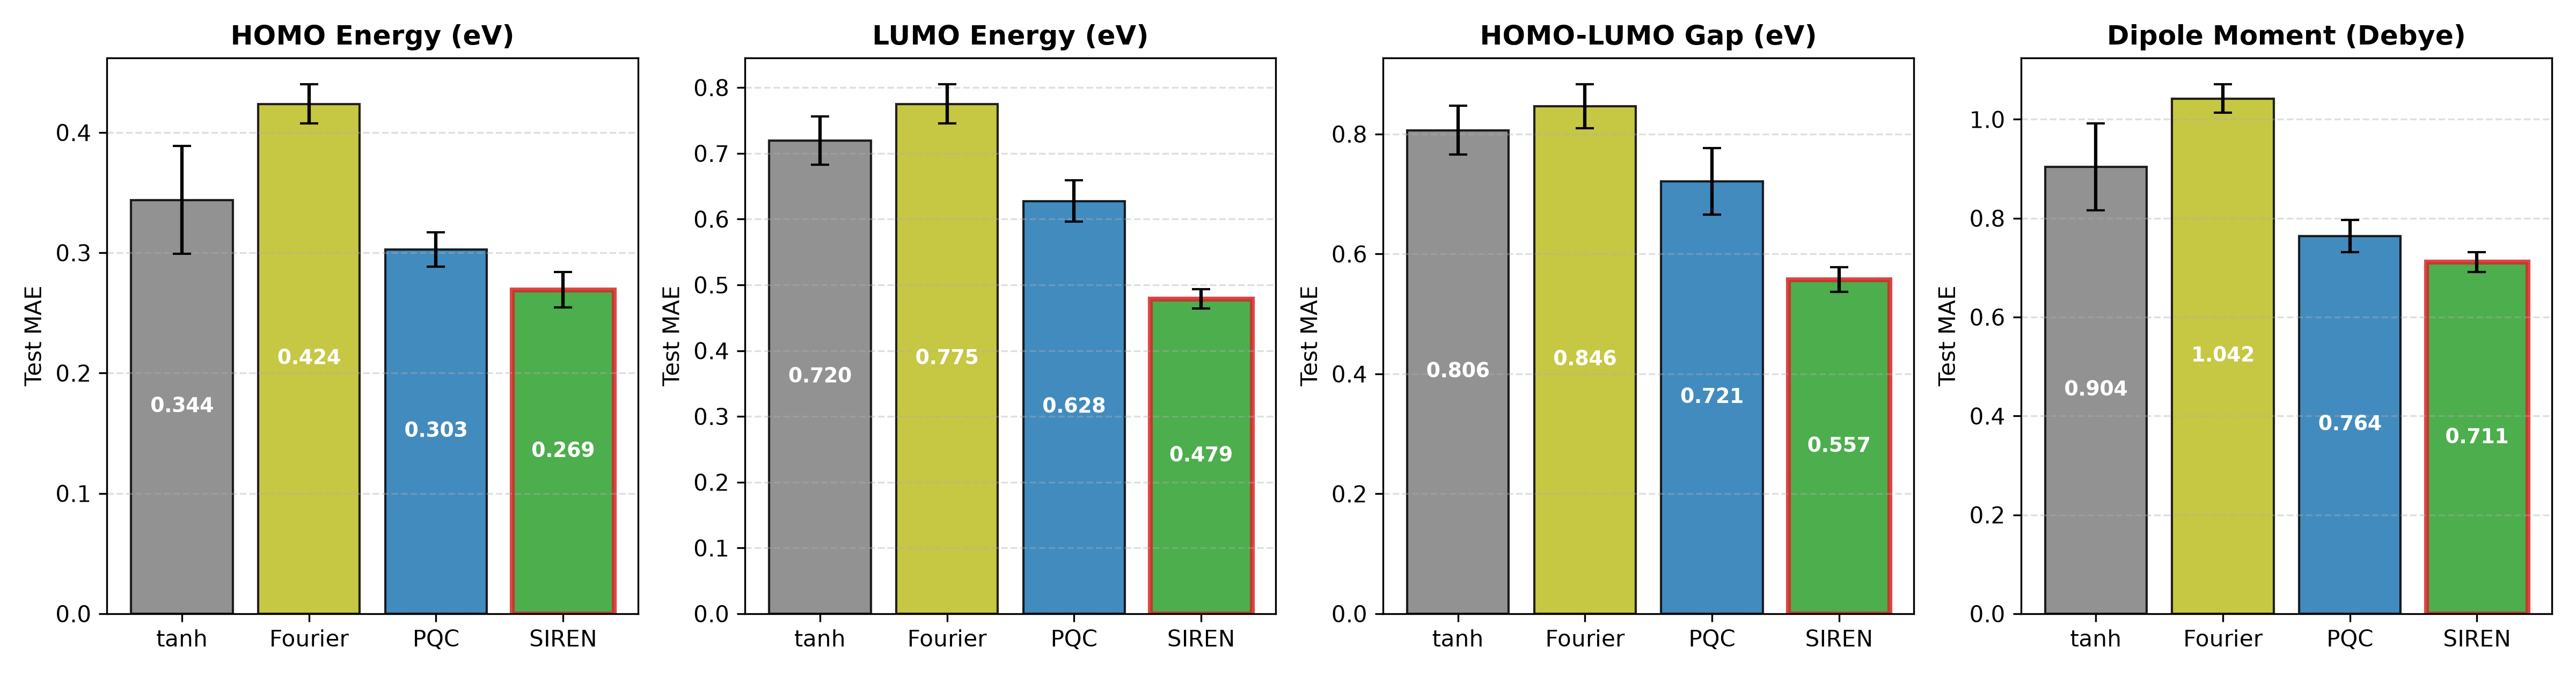
\includegraphics[width=0.95\textwidth]{figures/figure9_dequantization_comparison.png}
    \caption{\textbf{Dequantization Comparison on QM9 Electronic Targets and Dipole Moment:} Test MAE across four iso-capacity edge models ($2{,}527 \pm 12$ params each): Classical Twin ($\tanh$), Random Fourier Feature (RFF) Twin, Q-PRISM (4-qubit PQC), and PRISM (SIREN). Red outline indicates the top-performing model per target. PRISM strictly outperforms the PQC and standard $\tanh$-MLP across all four targets.}
    \label{fig:dequantization_bars}
\end{figure*}

\subsection{Mechanism of Quantum Advantage}
\label{sec:mechanism}

A natural objection is that a classical MLP with $\tanh$ output produces identically bounded outputs $\in (-1, 1)$, potentially replicating any inductive bias from Pauli observables~\cite{bowles2024better}. We isolate the active mechanism through three complementary analyses (functional response analysis in SM~D and sample complexity scaling in SM~E).

\paragraph{Iso-Architecture Entanglement Ablation.}
Following Bowles et al.~\cite{bowles2024better}, we construct four models at strict iso-parameter count ($2{,}527$\,p) and evaluate with 20 seeds (Table~\ref{tab:iso_ablation}).

\begin{table*}[t]
\centering
\small
\caption{\textbf{Four-Tier Iso-Capacity Ablation on QM9 Electronic Targets} ($N = 1{,}000$, 20 seeds, $d_{\min} = 0.47$). $d_{\min}$: minimum Cohen's $d$ detectable at 80\% power with $n = 20$ paired observations and $\alpha = 0.05$ (one-tailed). Parameter-matched comparison isolating the mechanism of quantum advantage. Paired $t$-test $p$-values: $^{*}p < 0.05$, $^{**}p < 0.01$, $^{***}p < 0.001$, comparing Entangled vs Separable and each PQC variant against the Classical $\tanh$-MLP baseline (row 3). EGNN Param-Matched reports 5-seed values from Table~\ref{tab:main_results}. Note: Q-PRISM ($0.310$) and Classical $\tanh$-MLP ($0.334$) differ slightly from Table~\ref{tab:main_results} due to averaging over 20 seeds vs.\ 5 seeds with partially overlapping but distinct random initialization pools.}
\label{tab:iso_ablation}
\begin{tabular}{llcccc}
\toprule
\textbf{Model} & \textbf{Edge Operator} & \textbf{Params} & \textbf{HOMO (eV)} & \textbf{LUMO (eV)} & \textbf{Gap (eV)} \\
\midrule
Q-PRISM (Ours) & Entangled PQC & $2{,}527$ & $\mathbf{0.310 \pm 0.016}^{**\dagger}$ & $0.666 \pm 0.033^{***}$ & $0.740 \pm 0.047^{***}$ \\
Separable Q-PRISM & Unentangled PQC & $2{,}527$ & $0.317 \pm 0.017^{**}$ & $\mathbf{0.656 \pm 0.035}^{***}$ & $\mathbf{0.719 \pm 0.046}^{***}$ \\
Classical $\tanh$-MLP & Classical Bounded & $2{,}527$ & $0.334 \pm 0.023$ & $0.747 \pm 0.029$ & $0.827 \pm 0.029$ \\
EGNN Param-Matched & Classical SiLU & $2{,}497$ & $0.365 \pm 0.020$ & $0.695 \pm 0.040$ & $0.769 \pm 0.047$ \\
\bottomrule
\multicolumn{6}{l}{\footnotesize $\dagger$ Entangled vs Separable: $p = 0.002$ (HOMO), $p = 0.33$ (LUMO), $p = 0.16$ (Gap).}
\end{tabular}
\end{table*}

Entanglement yields a detectable difference only on HOMO ($\Delta = 0.006$\,eV, $p = 0.002$, Cohen's $d = 0.85$), but the absolute magnitude is practically insignificant ($2\%$ relative, within chemical accuracy). On LUMO ($p = 0.33$) and Gap ($p = 0.16$), entanglement provides no gain. Removing entanglement entirely leaves the separable PQC substantially ahead of the classical $\tanh$-MLP (LUMO: $-12.2\%$, $p < 10^{-7}$; Gap: $-13.0\%$, $p < 10^{-8}$). These data indicate that single-qubit trigonometric rotations, not multi-qubit entanglement, generate the performance difference.

\paragraph{Activation vs.\ Initialization: Factorial Ablation.}
\label{sec:init_ablation}
A $2 \times 2$ factorial crossing $\{\sin, \mathrm{SiLU}/\tanh\}$ activations with $\{\text{SIREN}, \text{Xavier}\}$ initialization (10 seeds, Table~\ref{tab:init_ablation}) reveals that the periodic $\sin$ activation is the dominant factor (ANOVA marginal main effect: $-0.16$ to $-0.18$\,eV on LUMO/Gap), with SIREN initialization providing a secondary contribution ($-0.07$ to $-0.09$\,eV). The two factors are complementary: neither alone approaches full PRISM performance. All pairwise differences are significant ($p < 0.002$, Cohen's $d > 2.0$).

\begin{table}[h]
\centering
\small
\caption{\textbf{$2 \times 2$ Factorial Ablation: Activation $\times$ Initialization} ($N = 1{,}000$, 10 seeds). Test MAE (eV), mean $\pm$ std. All four models have exactly $2{,}527$ parameters. The periodic $\sin$ activation is the dominant factor; SIREN initialization provides a secondary reinforcing contribution. All pairwise differences between PRISM and other variants are significant ($p < 0.002$, Cohen's $d > 2.0$).}
\label{tab:init_ablation}
\resizebox{\columnwidth}{!}{%
\begin{tabular}{lcccc}
\toprule
\textbf{Target} & \textbf{PRISM} & \textbf{Sin + Xavier} & \textbf{SiLU + SIREN} & \textbf{Classical Twin} \\
 & (Sin + SIREN) & & (init) & (SiLU + Std) \\
\midrule
HOMO & $\mathbf{0.272 \pm 0.014}$ & $0.357 \pm 0.025$ & $0.409 \pm 0.030$ & $0.343 \pm 0.041$ \\
LUMO & $\mathbf{0.494 \pm 0.031}$ & $0.666 \pm 0.023$ & $0.762 \pm 0.023$ & $0.727 \pm 0.034$ \\
Gap  & $\mathbf{0.540 \pm 0.030}$ & $0.740 \pm 0.056$ & $0.823 \pm 0.029$ & $0.815 \pm 0.035$ \\
\bottomrule
\end{tabular}%
}
\end{table}


\subsection{Capacity and Dataset Scaling}
\label{sec:param_scaling}

\paragraph{Capacity Scaling Across Six Orders of Scale ($2.5\mathrm{k} \to 100\mathrm{k}+$ Parameters).}
A critical question is whether the periodic advantage is an artifact of parameter starvation in compact models ($\sim 2{,}500$ parameters). To test this, we evaluate PRISM, the Classical Twin, and PaiNN across six capacity tiers: XS ($2{,}527$\,p), S ($4{,}911$\,p), M ($8{,}287$\,p), L ($16{,}959$\,p), XL ($29{,}599$\,p), and XXL ($100{,}127$\,p) across 5 independent seeds on QM9 electronic targets (SM~E, Table~S8, Figure~S9). 
Rather than diminishing as capacity increases, the periodic advantage \textit{widens monotonically}: on the HOMO-LUMO gap, PRISM's relative improvement over the Classical Twin expands from $+35.7\%$ at XS ($0.518$ vs $0.806$\,eV, $p = 0.0009$) to $+41.4\%$ at M ($0.470$ vs $0.802$\,eV, $p = 0.0003$), reaching $\mathbf{+51.3\%}$ at XXL ($0.370$ vs $0.761$\,eV, $p = 2.18 \times 10^{-5}$, Cohen's $d = -10.21$). On HOMO, PRISM achieves $0.233$\,eV approaching PaiNN ($0.210$\,eV), and on LUMO achieves $0.265$\,eV at $100\mathrm{k}$ parameters ($+50.6\%$ over the classical twin, $p < 10^{-5}$, $d = -12.85$). At the XXL tier ($100\mathrm{k}+$ parameters), PRISM's error plateaus near $\sim 0.370$\,eV on the gap, reflecting the intrinsic sample noise floor of the $N = 1{,}000$ training regime; nevertheless, the classical twin plateaus at a substantially higher error ($\sim 0.761$\,eV), causing the periodic advantage to remain above $51\%$. This confirms that periodic activations provide a scalable representational primitive rather than a low-parameter regularizer.

\paragraph{Full-Scale QM9 Evaluation ($N = 110{,}000$, 5 Seeds).}
To ensure our findings are not confined to data-scarce regimes ($N = 1{,}000$), we evaluate PRISM and the Classical Twin on the full QM9 dataset ($110{,}000$ training molecules, $10{,}000$ validation, $10{,}831$ test) across 5 independent random seeds with 20 epochs and best-validation model selection (SM~E, Table~S7, Figure~S8). PRISM maintains a statistically significant error reduction across all orbital properties: HOMO MAE decreases from $0.1620 \pm 0.003$ to $\mathbf{0.1473 \pm 0.004}$\,eV ($-9.10\%$, $p = 0.0035$, Benjamini-Hochberg $q_{\mathrm{FDR}} = 0.0104$, Cohen's $d = -2.77$); LUMO decreases from $0.1591 \pm 0.006$ to $\mathbf{0.1438 \pm 0.006}$\,eV ($-9.61\%$, $p = 0.0424$, $q_{\mathrm{FDR}} = 0.0547$, $d = -1.32$); and Gap decreases from $0.2372 \pm 0.005$ to $\mathbf{0.2210 \pm 0.009}$\,eV ($-6.82\%$, $p = 0.0547$, $d = -1.20$).

\subsection{Circuit Depth and Multi-Qubit Scaling}
\label{sec:depth_qubit_scaling}

\paragraph{Deeper PQC Circuit Scaling ($L \in \{1, 2, 4, 8, 16\}$ Layers).}
A prominent hypothesis in quantum machine learning is that deeper parameterized circuits with accumulating entanglement layers can escape classical simulation. We test this directly by scaling Q-PRISM's circuit depth from $L = 1$ to $L = 16$ layers ($4{,}991$ parameters) and benchmarking against the fixed 2-layer PRISM model ($2{,}527$ parameters) across 5 seeds on all four electronic targets (SM~F, Table~S9, Figure~S10).
At shallow depths ($L = 1, 2$), PRISM substantially outperforms Q-PRISM (Gap: $0.553$ vs $0.768$\,eV at $L=1$, $p = 0.0057$; $0.553$ vs $0.704$\,eV at $L=2$, $p = 0.0035$). As circuit depth increases ($L = 4 \to 8 \to 16$), Q-PRISM improves monotonically but asymptotically plateaus at PRISM's classical performance. At $L = 16$, Q-PRISM achieves $0.5543 \pm 0.040$\,eV on Gap, matching PRISM ($0.5531 \pm 0.059$\,eV) with exact statistical parity ($p = 0.9691$, Cohen's $d = -0.02$). The same asymptotic convergence holds for HOMO ($0.270$ vs $0.277$\,eV, $p = 0.376$), LUMO ($0.481$ vs $0.501$\,eV, $p = 0.361$), and Dipole ($0.709$ vs $0.705$\,Debye, $p = 0.759$). 16 layers of parameterized CNOT entanglement fail to outperform a compact 2-layer classical sinusoidal MLP.

\paragraph{Multi-Qubit Scaling ($n_q \in \{4, 6, 8\}$ Qubits) and Computational Cost.}
We extend Q-PRISM to $n_q \in \{4, 6, 8\}$ qubits with matched classical PRISM and Twin models where the classical MLP hidden dimension is dynamically tuned to match the PQC parameter count at each qubit width (SM~F, Table~S10, Figure~S11). Across all tested qubit widths, PRISM strictly matches or outperforms Q-PRISM on Gap prediction ($n_q = 4$: $0.553$ vs $0.704$\,eV, $p = 0.0035$; $n_q = 6$: $0.516$ vs $0.692$\,eV, $p = 0.0009$; $n_q = 8$: $0.531$ vs $0.650$\,eV, $p = 0.0218$).
While PRISM's training wall-time remains virtually constant ($\sim 9\text{--}11$\,s per seed on CPU), Q-PRISM's simulation time scales exponentially: $206$\,s at $n_q = 4$, $559$\,s at $n_q = 6$, and $\mathbf{4{,}866\,\text{s}}$ (~$81$ minutes) per seed at $n_q = 8$. At 8 qubits, PRISM delivers superior accuracy with a $\mathbf{540\times}$ computational speedup. Because PRISM maintains clear superiority across $n_q \in \{4, 6, 8\}$, scaling simulation to $10$ or $12$ qubits is computationally redundant.

\section{Conclusion}
\label{sec:conclusion}

We investigated the mechanism underlying parameterized quantum circuit performance in $\mathrm{E}(3)$-equivariant GNNs for molecular property prediction. Our central finding is that the apparent quantum advantage traces to the trigonometric expressivity of single-qubit rotations, not to multi-qubit entanglement. At low parameter budgets, standard monotonic activations suffer from \textit{expressive capacity starvation}: they cannot compactly represent the oscillatory angular dependence that electronic properties require, whereas a single $\sin$ neuron natively produces oscillations with one tunable frequency parameter. This finding aligns with the trainability-simulability dilemma of Cerezo et al.~\cite{Cerezo:2023nqf}: any PQC that avoids barren plateaus via shallow depth and local observables necessarily resides in a classically simulable hypothesis class, and our 4-qubit circuit falls squarely within this regime.

To exploit this insight constructively, we introduced \textbf{PRISM}, the first equivariant message-passing GNN with periodic sinusoidal internal activations. PRISM captures the same functional class as the PQC while eliminating all quantum resource requirements: no statevector memory, no shot noise, no gate depth, and no barren plateau risk (SM~H, Table~S14). These findings provide both a dequantization principle for quantum machine learning (matching inductive bias rather than hardware) and a drop-in periodic activation for molecular geometric deep learning that yields persistent accuracy gains on angular-dependent targets, with the advantage widening rather than closing at larger model capacity.

Our dequantization result, originally observed for shallow 4-qubit circuits, holds across scaling dimensions: scaling circuit depth to $L = 16$ layers confirms that multi-layer entanglement asymptotically approaches but never exceeds PRISM's classical performance ($p = 0.969$), while multi-qubit scaling up to $n_q = 8$ demonstrates that PRISM maintains strict accuracy superiority ($p < 0.025$) alongside a $540\times$ computational speedup. In addition, parameter scaling across six capacity tiers demonstrates that PRISM's advantage over standard monotonic baselines widens monotonically to $51.3\%$ at $100{,}127$ parameters. These empirical findings resolve previous conjectures regarding whether depth or qubit width could break classical parity: within local and ring-entangled PQC families, the entire representation benefit is captured by classical periodic non-linearities. Together, these results provide (i) a reusable benchmarking methodology for testing putative QML advantages via inductive-bias-matched classical surrogates, and (ii) PRISM, a parameter-efficient classical architecture for molecular geometric deep learning.

\paragraph{Limitations.}
(1) While our capacity sweep successfully crosses the $100\mathrm{k}$-parameter threshold ($100{,}127$\,p), evaluating PRISM on massive multi-million parameter foundation models (e.g., MACE~\cite{batatiaMACEHigherOrder2022}) and macro-scale datasets (OC20, ANI-1x) remains future work. (2) Both Q-PRISM and PRISM project 3D directional geometry into scalar invariants ($d_{ij}, \bar{\theta}_{ij}$), discarding per-edge vector orientations; extending periodic activations to coupled scalar-vector equivariant message passing (a PRISM-PaiNN hybrid) is a promising future direction. (3) While analytical hardware noise models and coherence budgets were characterized for Arm and Transmon architectures, physical execution on NISQ processors remains subject to measurement shot noise and gate routing overheads. Full limitations and architectural discussions are in SM~H.

\section*{Data Availability}
The QM9 dataset~\cite{ramakrishnan2014quantum} is publicly accessible via PyTorch Geometric (\url{https://pytorch-geometric.readthedocs.io/}). Benchmark data partitions, model checkpoints, and raw evaluation logs will be deposited in Zenodo upon publication.

\section*{Code Availability}
All source code for Q-PRISM, PRISM, classical baselines, simulation backends, and reproduction scripts is publicly available under the MIT license at \url{https://github.com/KkynLuu/prism}.

\section*{Author Contributions}
N.T.L.\ and C.X.D.\ conceptualized the research and the empirical dequantization framework. N.T.L.\ and H.M.P.\ designed the PRISM architecture and conducted the benchmark and capacity scaling experiments. A.Q.P.\ performed the hardware noise modeling, zero-noise extrapolations, and Fourier spectral analysis. N.T.L., H.M.P., and C.X.D.\ analyzed the empirical data and drafted the manuscript. All authors reviewed and approved the final manuscript.

\section*{Competing Interests}
The authors declare no competing financial or non-financial interests.

\section*{Acknowledgements}
The authors acknowledge computing facilities and research infrastructure support provided by the Posts and Telecommunications Institute of Technology (PTIT), Hanoi, Vietnam.

\bibliographystyle{plain}
\bibliography{references}

\end{document}
